
% this file is called up by thesis.tex
% content in this file will be fed into the main document

%: ----------------------- introduction file header -----------------------
%\begin{savequote}[50mm]
%Now this is not the end. It is not even the beginning of the end. But it is, perhaps, the end of the beginning. 
%\qauthor{Winston Churchill}
%\end{savequote}


\chapter{Conclusiones y trabajo futuro}
\label{cha:Conclusions}

% the code below specifies where the figures are stored
\ifpdf
    \graphicspath{{6_conclusion/figures/PNG/}{6_conclusion/figures/PDF/}{6_conclusion/figures/}}
\else
    \graphicspath{{6_conclusion/figures/EPS/}{6_conclusion/figures/}}
\fi


En este capítulo se presentan las conclusiones de este trabajo de investigación, y se comentan los trabajos futuros que se derivan del mismo.

%------------------------------------------------------------------------- 

\section{Conclusiones}

En esta tesis doctoral se estudia la utilización de indicadores procedentes de los registros de actividades de aprendizaje para evaluar las competencias genéricas de los estudiantes que participan en dichas actividades.

Para alcanzar los objetivos enunciados en el capítulo introductorio se propuso un método de evaluación denominado design-based assessment (DBA) y se desarrollaron dos lenguajes específicos de dominio (DSL). El método DBA permite definir una hipótesis de evaluación mediante el diseño de indicadores a partir de la información de los registros de actividad de los estudiantes en entornos virtuales de aprendizaje, para después analizar los resultados de su aplicación, y si el docente lo considera necesario, redefinir la hipótesis inicial comenzando de nuevo el ciclo. SASQL y VWQL son los DSL que se han desarrollado para facilitar la aplicación del método en cursos virtuales basados en Moodle y en mundos virtuales basados en OpenSim respectivamente.

Para la evaluación tanto del método como de los DSL desarrollados se plantearon las siguientes hipótesis: el método DBA permite obtener de manera automática indicadores de los entornos virtuales de aprendizaje (H1) y los DSL permiten a los docentes diseñar y contrastar estrategias de evaluación a partir de los registros de actividad de los entornos virtuales de aprendizaje (H2).

Para contrastar dichas hipótesis, el método DBA junto con los DSL se han aplicado y utilizado, en primer lugar, a varias asignaturas del Grado en Ingeniería Informática de la Universidad de Cádiz y en un estudio de caso llevado a cabo en un curso de idiomas con estudiantes de instituto. En segundo lugar, ambos fueron evaluados por docentes de todos los niveles educativos y pertenecientes a todas las ramas de conocimiento.

De los resultados de la evaluación realizada, se deriva que el método DBA permite abordar la evaluación de competencias genéricas, ya que aporta indicadores objetivos del trabajo de los estudiantes en los entornos virtuales que han sido evaluados positivamente en el estudio.

En concreto, hay evidencias a favor de las siguientes conclusiones:

\begin{itemize}
\item El método de evaluación DBA es adecuado para diseñar y contrastar estrategias de evaluación a partir de los registros de actividades de los entornos virtuales de aprendizaje. Las características del método DBA más valoradas en el estudio realizado son su adaptabilidad, su sistematicidad y su flexibilidad. 
\item El DSL facilita la implementación del método DBA. Las características del DSL más valoradas son su facilidad de aprendizaje, su eficacia, su eficiencia y su capacidad de reutilización. Además, tanto las consultas que se pueden definir con el DSL como los resultados que el sistema devuelve fueron fácilmente interpretables por la mayoría de la población encuestada, lo que evidenció que el DSL puede ser utilizado por docentes sin conocimientos de programación.
\end{itemize}
% ----------------------------------------------------------------------

\subsection{Alcance}

El alcance de las conclusiones anteriormente mencionadas se deben considerar cuando concurran situaciones similares a las descritas en este trabajo de investigación. Sin embargo, no se puede confirmar que una situación quede dentro del alcance de las mismas cuando se den circunstancias como las que se describen a continuación:

\begin{itemize}
\item Los docentes no incorporen en sus cursos virtuales módulos que generen actividad en los registros de aprendizaje o, si aún teniendo dichos módulos, no fomentan su utilización entre los estudiantes del curso.
\item No se disponga de acceso a los registros que contienen la información de la actividad generada por los estudiantes en los entornos virtuales de aprendizaje ni mediante conexión directa ni mediante copia de seguridad. En este caso podría aplicarse un método basado en Linked Open Data~\cite{ruiz2015framework} para convertir en abiertos los datos alojados en el entorno virtual de aprendizaje. 
\end{itemize}

\subsection{Amenazas a la validez}

% ~\cite{oates2006researching} capítulo 7
La principal amenaza a la validez es que el método DBA y los DSL han sido probados y evaluados en una muestra adecuada en tamaño~\cite{oates2006researching} pero limitada. En concreto, la mayoría eran docentes que, aunque no tengan perfil informático, tienen en común su interés por la innovación educativa, las nuevas tecnologías y su aplicación en la mejora de los procesos de aprendizaje. Los foros en los que han conocido tanto el método DBA como los DSL son congresos, seminarios y cursos a los que fueron por propia voluntad. Por tanto, quedaría conocer la experiencia de docentes que a priori no tienen estas inquietudes y/o suelen quedarse al margen de estos eventos.

Por otro lado, también se considera una amenaza a la validez el hecho de que el método DBA, mediante las herramientas implementadas, se ha probado únicamente en dos entornos virtuales de aprendizaje concretos: en el sistema de gestión de aprendizaje Moodle (mediante SASQL) y en mundos virtuales basados en OpenSim (mediante VWQL). Habría que adaptar los DSL para que sean utilizables en el análisis de las interacciones producidas en otros entornos virtuales de aprendizaje tales como plataformas de desarrollo colaborativo, repositorios de contenidos digitales y aplicaciones de realidad aumentada.

\section{Contribuciones} \label{eva:contribuciones}

	A continuación se indican las aportaciones principales que se han realizado durante la elaboración de este trabajo de investigación:

	\subsection*{Publicaciones en revistas}


Artículo en la revista Computers in Human Behavior (2014), titulado ``\textbf{Scalability of assessments of wiki-based learning experiences in higher education}''~\cite{palomo2014scalability} (\emph{ISI JCR 2014: Q1, T1})

\begin{quote}En este artículo se presentaron siete estudios de caso de evaluación de wikis en educación superior. Entre esas experiencias destacan dos que hacían uso de herramientas para abordar de manera escalable la evaluación de varias habilidades de los estudiantes a partir del trabajo realizado en wikis de MediaWiki. Se analizaron y compararon las diferentes metodologías y configuraciones de las herramientas utilizadas en el contexto de cada uno de los siete estudios de caso aportados. Una de las herramientas que se utilizaron fue AssessMediaWiki, que mediante procedimientos de autoevaluación, hetero-evaluación y evaluación entre iguales complementó con una visión cualitativa el enfoque cuantitativo aportado por la herramienta StatMediaWiki.\end{quote}

\noindent
Artículo en la revista International Journal of Engineering Education (2015), titulado ``\textbf{A Domain Specific Language for Online Learning Competence Assessments}''~\cite{Balderas:2015} (\emph{ISI JCR 2014: Q3, T3})

\begin{quote}En este artículo se utilizó SASQL para el diseño de evaluaciones a partir de indicadores obtenidos de la interacción de los estudiantes en dos estudios de caso basados en dos cursos virtuales. Estos indicadores se utilizaron para asistir en la evaluación del desempeño de los estudiantes en las competencias genéricas del liderazgo, las habilidades interpersonales y la habilidad para ser crítico y autocrítico.\end{quote}

\noindent
Artículo enviado a la revista Journal of Information Technology Research (2016) tras ser invitados por una contribución previa en el congreso TEEM 2015, titulado ``\textbf{Retrieving Objective Indicators from Student Logs in Virtual Worlds}'' (SCImago SJR 2014: Q4)

\begin{quote}En este artículo se analiza el comportamiento de los estudiantes en un mundo virtual basado en OpenSim mediante el uso de EvalSim y VWQL. Se diseñaron evaluaciones y se obtuvieron indicadores del desempeño de los estudiantes a partir de su interacción en el mundo virtual. Estos indicadores se utilizaron para establecer una comparación más justa del rendimiento de los estudiantes y sacar conclusiones sobre el análisis del proceso de aprendizaje.\end{quote}

%\fcolorbox{grey}{grey}{\parbox{0.7\textwidth}{%
%   \color{black}%
% % Para cuadro gris
%}}

	\subsection*{Contribuciones/Comunicaciones a congresos}

Comunicación presentada en el congreso \emph{IX Simposio Pluridisciplinar sobre Diseño, Evaluación y Descripción de Contenidos Educativos (SPDECE 2012)}, titulada ``\textbf{Qualitative assessment of wiki-based learning processes}''~\cite{Balderas:2012}

\begin{quote}	En esta contribución se presentó AssessMediaWiki y se aplicó con el fin de dar soporte a procedimientos de autoevaluación y evaluación entre iguales. Estos procedimientos se utilizaron en la evaluación de las contribuciones realizadas por los estudiantes a un wiki basado en MediaWiki. Los estudiantes evaluaron las contribuciones de sus iguales a partir de los aspectos de una rúbrica sobre el trabajo específico que estos debían realizar, mientras que el docente utilizó dichas evaluaciones para evaluar la capacidad críticas de sus estudiantes.\end{quote}

\noindent
Comunicación en forma de póster presentada en el \emph{8th European Conference on Technology Enhanced Learning (EC-TEL 2013)}, titulada ``\textbf{A generative computer language to customize online learning assessments}''~\cite{Balderas:2013}

\begin{quote}En esta contribución se presentaron la herramienta EvalCourse y la sintaxis del lenguaje SASQL junto con un sencillo ejemplo.\end{quote}

\noindent
Comunicación presentada en el \emph{4th International Workshop on Software Engineering for E-learning (ISELEAR’13)}, dentro del \emph{I International Conference on Technological Ecosystem for Enhancing Multiculturality (TEEM 2013)}, titulada ``\textbf{A generative computer language to customize online learning assessments}''~\cite{balderas2013generative}

\begin{quote}En esta contribución se presentaron EvalCourse y SASQL, y se aplicaron a un estudio de caso para extraer indicadores de la actividad de los estudiantes del campus virtual de una asignatura. Estos indicadores se utilizaron para asistir en la evaluación del desempeño de estos en las competencias genéricas del liderazgo, la planificación y gestión del tiempo y el trabajo en equipo.\end{quote}

\noindent
Comunicación presentada en el \emph{Simposio Internacional de Informática Educativa (SIIE 2014)}, titulada ``\textbf{Domain-driven competence assessment in virtual learning environments. Application to planning and time management skills}''~\cite{balderas2014domain}

\begin{quote}En esta contribución se compararon dos alternativas para abordar la problemática de la evaluación de competencias genéricas. La primera alternativa se basa en una arquitectura dirigida por modelos en la que se utiliza EvalCourse y SASQL, mientras que la segunda alternativa se basa en Gescompeval\_MD, un servicio Web ReST que permite al docente indicar las competencias que desarrollarán los estudiantes mediante cada actividad. Los resultados de aplicar conjuntamente ambos enfoques mostraron que son complementarios, ya que mientras el servicio web proporciona una retroalimentación mucho más detallada, el enfoque dirigido por modelos es más escalable cuando el número de estudiantes es elevado y hay que evaluar competencias genéricas.\end{quote}

\noindent
Comunicación presentada en el \emph{6th International Workshop on Software Engineering for E-learning (ISELEAR’15)}, dentro del \emph{III International Conference on Technological Ecosystem for Enhancing Multiculturality (TEEM 2015)}, titulada ``\textbf{A Domain Specific Language to retrieve objective indicators for foreign language learning in virtual worlds}''~\cite{balderas2015domain}

\begin{quote}En esta contribución se presentó VWQL, así como una experiencia piloto de aplicación en el mundo virtual utilizado en un curso de idiomas. Se diseñaron evaluaciones a partir de indicadores de las interacciones de los estudiantes en el mundo virtual. Estos indicadores se aplicaron en la evaluación de la competencia genérica de la habilidad para comunicarse en lengua extranjera.\end{quote}


	\subsection*{Otras contribuciones}

	A continuación se describen otras contribuciones que resultan del trabajo desarrollado en esta tesis doctoral y que no se recogen en los apartados anteriores. Estas contribuciones se dividen en dos categorías principales. La primera es la de \emph{contribuciones metodológicas}, categoría en la que se enmarca el método de evaluación propuesto. Mientras que la segunda de las categorías es la de \emph{contribuciones en forma de software}, que engloba las diferentes herramientas desarrolladas para poner en práctica el método.

	\paragraph*{Contribuciones metodológicas}

	\begin{itemize}
	\item Método DBA: método de evaluación basado en el diseño de indicadores a partir de la información del registro de actividad de los entornos virtuales de aprendizaje.
	\end{itemize}

	\paragraph*{Contribuciones en forma de software}

	\begin{itemize}
	\item Sistema AssessMediaWiki~\cite{Balderas:2012}: herramienta web que asiste en procedimientos de evaluación entre iguales y autoevaluación de las contribuciones realizadas por los estudiantes en un wiki basado en MediaWiki.
	\item Sistema EvalCourse y lenguaje de consultas SASQL~\cite{Balderas:2013,balderas2013generative,Balderas:2015}: DSL para la aplicación del método DBA en cursos virtuales basados en Moodle.
	\item Sistema EvalSim y lenguaje de consultas VWQL~\cite{balderas2015domain}: DSL para la aplicación del método DBA en mundos virtuales basados en OpenSim.

	\end{itemize}

\section{Trabajo futuro}

Durante la realización de este trabajo se han superado los retos que se plantearon inicialmente. Sin embargo, se han encontrado algunos problemas o nuevos retos que no han llegado a ser abordados pero que complementarían en muchos casos esta tesis doctoral.

Estos trabajo futuros son:
\begin{itemize}
\item Adaptar y ampliar los DSL que se han presentado en esta tesis para que puedan ser utilizados en la obtención de indicadores de otros entornos virtuales de aprendizaje tales como plataformas de desarrollo colaborativo, repositorios de contenidos digitales, y aplicaciones de realidad aumentada.
\item Añadir indicadores basados en la aplicación de técnicas de análisis de redes sociales (SNA, del inglés \emph{Social Network Analysis}) a los entornos virtuales de aprendizaje. En un wiki de Moodle utilizado en clase se puso a los estudiantes en parejas para que cada pareja realizase su trabajo en una página del wiki. Una vez finalizada la actividad, aplicando técnicas de SNA se obtuvo el grafo que se muestra en la figura 1. En dicho grafo, el nodo central es el docente. Puede verse cómo al principio el docente creó la sección principal, mientras que los estudiantes ubicaron los enlaces a sus páginas en dicha página principal (arista que une a los nodos periféricos con el nodo central). El resto de aristas que unen normalmente dos nodos periféricos representan los estudiantes que colaboraron juntos en una página. El tamaño de los nodos representa la cantidad de trabajo realizado por cada estudiante. Los indicadores obtenidos mediante este análisis podrían ser aplicados en la evaluación de competencias genéricas relacionadas con el trabajo y la interacción de equipos.
\end{itemize}

\begin{figure}[h]
  \begin{center}
    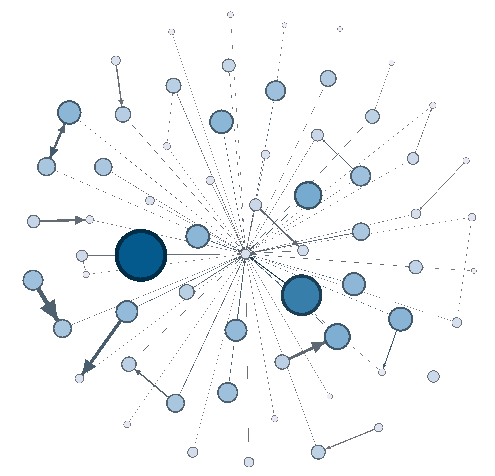
\includegraphics[scale=0.5]{SNA-Grafo-Wiki-SD.png}
  \end{center}
  \caption{Grafo resultante de aplicar técnicas de SNA a un wiki de Moodle}
  \label{fig:SNAWiki}
\end{figure}

\begin{itemize}
\item Integrar los DSL con los propios entornos virtuales de aprendizaje. Los DSL que se han presentado en este trabajo no están integrados en los entornos virtuales, sino que se conectan a ellos para obtener los indicadores. En ocasiones, la configuración de esta conexión puede resultar una tarea compleja para docentes con pocos conocimientos informáticos, por lo que sería interesante poder integrar el DSL en los entornos dentro del perfil de supervisor. Para hacerlo se podría utilizar en el servidor la última versión de Xtext, ya que incorpora XtextServlet para responder a las peticiones de los clientes y así poder implementar el parser del lenguaje para su uso a través de HTTP. En la parte del cliente se podría utilizar un editor web hecho en JavaScript (CodeMirror~\footnote{\url{http://codemirror.net}}, Orion~\footnote{\url{https://orionhub.org}}, etc.).
\item Crear una versión visual del DSL. A pesar de haber tratado de desarrollar un lenguaje sencillo con una sintaxis cercana al dominio de la docencia, puede haber docentes que sigan sin encontrarse cómodos a la hora de programar las consultas. En este caso, una versión visual del DSL podría ser más atractiva para docentes con este perfil. Para desarrollar el DSL visual se podría estudiar su implementación mediante la herramienta Eclipse Sirius~\footnote{\url{https://eclipse.org/sirius}}.
\item Establecer un repositorio que relacione actividades a realizar por los estudiantes en los entornos virtuales de aprendizaje, indicadores que se generan y competencias genéricas que se evaluarían con dichos indicadores. Los docentes que han aplicado la herramienta han ido proponiendo indicadores para evaluar competencias. Si los usuarios del método publican sus hipótesis de evaluación de competencias a partir de indicadores, la comunidad de docentes podría aprovecharse de estos indicadores para ver cómo lo hacen otros docentes y evaluar a sus estudiantes en estas competencias a partir de dichas hipótesis tal cuál están o mediante la redefinición de las mismas.
\end{itemize}


% ----------------------------------------------------------------------
